% !TEX root = 00_arbeit.tex

%---------------------------------------------------------------------------------
%% Anhang

%-------------------------------------------
%% Resettet den Abbildungszähler
%% Quelle:https://stackoverflow.com/questions/3391540/renumbering-figure-in-latex
\makeatletter 
\renewcommand{\thefigure}{A-\@arabic\c@figure}
\renewcommand{\theequation}{A\@arabic\c@equation} 
\makeatother
\setcounter{figure}{0}
\setcounter{equation}{0}

\section{Anhang}

\subsection{XOR bzw. exklusiv Oder}\label{sec:XOR}

\begin{figure}[!h]
\centering
\begin{circuitikz}
\draw (0,0)         node[european xor port] (xor)   {} 
      (xor.in 1)    node[left]                      {A}
      (xor.in 2)    node[left]                      {B}
      (xor.out)     node[right]                     {Y}
      ;
\end{circuitikz}
%\includegraphics{test}
\hspace{1cm}
\begin{tabular}{cc|c}
A & B & Y \\
\hline
0& 0 & 0 \\
0& 1 & 1 \\
1& 0 & 1 \\
1& 1 & 0 
\end{tabular}
\caption[Blockschaltbild des XOR-Gatters]{Blockschaltbild des XOR-Gatters links und rechts die zugehörige Wahrheitstabelle.}
\label{fig_a:XOR}
\end{figure}

Das exklusive Oder bzw. XOR-Gatter ist ein Begriff aus dem Bereich der Logik. Mit der Gleichung:%
%
%$$Y=\left ( \overline{A}  \land B \right)\lor \left ( A \land \overline{B} \right ).$$
\begin{equation}
Y=\left ( \overline{A}  \land B \right)\lor \left ( A \land \overline{B} \right ).
\end{equation}
Der Ausgang dieses Gatters ist dann~\glqq 1\grqq~wenn eine ungerade Anzahl an Eingängen auf~\glqq 1\grqq~liegt und die restlichen auf~\glqq 0\grqq. Das Blockschaltbild und die Wahrheitstabelle sind in \autoref{fig_a:XOR} dargestellt.




\subsection{Gradientenabstiegsverfahren}\label{sec:gradient}

\begin{figure}[tb]
    \centering
        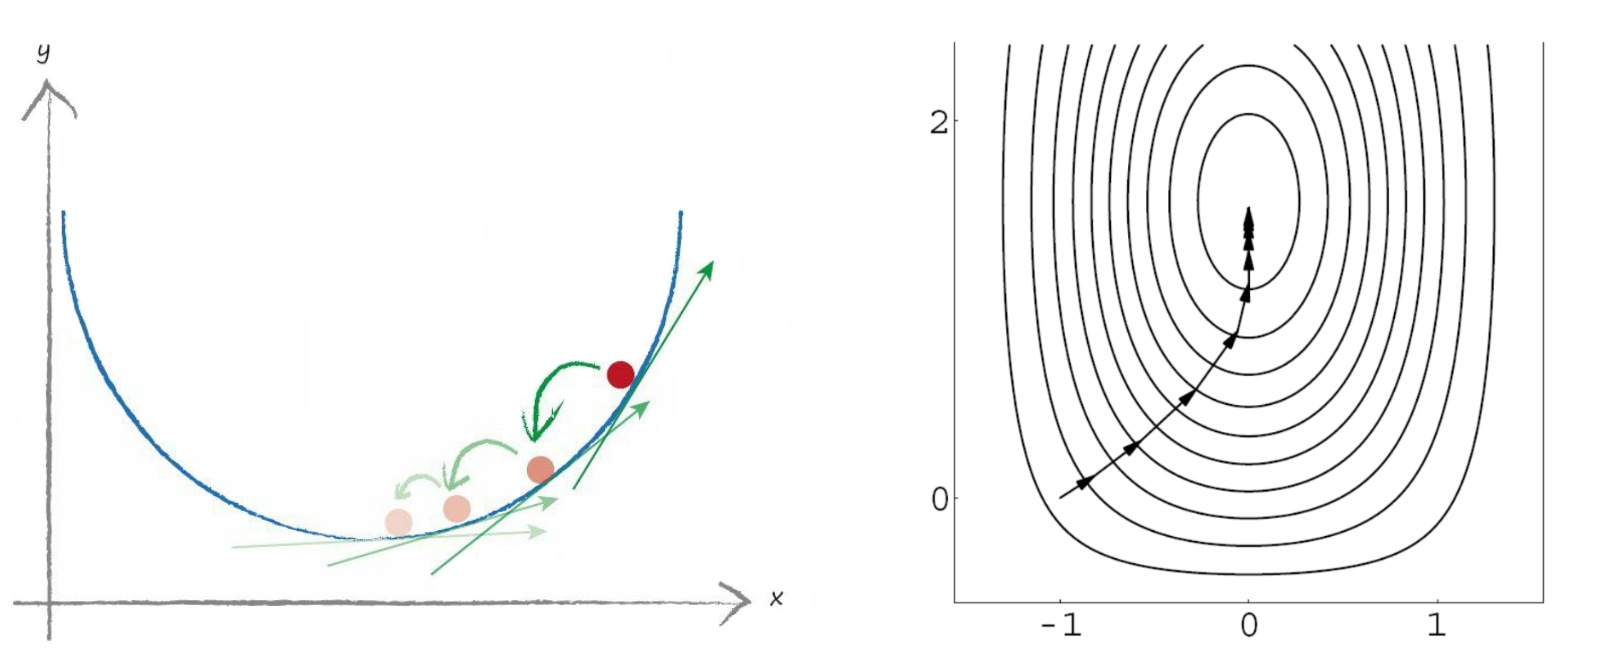
\includegraphics[width=0.9\textwidth]{Bilder/misc/Gradientenabstieg.png}
    \caption[Gradientenabstieg]{Gradientenabstieg bei einer 2-dimensionalen Funktion links und rechts bei einer 3-dimensionalen Funktion.\protect\footnotemark{}}
    \label{fig:gradient}
\end{figure}
\addtocounter{footnote}{-1}     %  -1 mal die Gesamtanzahl an Fußnoten in der wrapfigure
\addtocounter{Hfootnote}{-1}    % -1 times total number of footnote(mark)s in the wrapfigure
\wrapfigfoot\footnotetext{\autoref{fig:gradient} links wurde aus \citet{Rashid2016} Abbildung 1-80 angepasst und rechts wurde aus \citet[64]{dkriesel07} Abbildung 4.3 übernommen.}

Der Gradientenabstieg (engl.: gradient descent) ist ein Verfahren welches eingesetzt wird, um Maxima oder Minima einer Funktion zu finden. Der Gradient $g$ ist hierbei ein Vektor der an jedem Punkt einer differenzierbaren Funktion definiert ist. Der Vektor zeigt in Richtung des steilsten Anstieges und sein Betrag $|g|$ gibt den Steigungsgrad in diese Richtung an. Hieraus folgt, dass ein negativer Gradient $-g$ die Richtung des steilsten Abstieges weist. Bei dem Gradientenabstig wird von einem beliebigen Startpunkt einer Funktion schrittweise in die Richtung des negativen Gradienten gegangen, um das Minimum einer Funktion zu finden.\,\citef[63 ff]{dkriesel07} In \autoref{fig:gradient} wird dieses Verfahren anhand einer 2- und 3-dimensionalen Funktion veranschaulicht.

%\todo{sagen dass die Delta-Regel ein Gradientenabstiegsverfahren ist und das Verfahren beschreiben}

\subsection{Deltaregel}\label{sec:deltaregel}
%\todo{Perceptron-Lernalgorithmus}
    %http://www.theprojectspot.com/tutorial-post/introduction-to-artificial-neural-networks-part-2-learning/8

%\todo{Grafik: SLP mit Linearer Aktivierungsfunktion und Abkürzungsübersicht}
Die Deltaregel basiert auf dem Graientenabstiegsverfahren und wird als Lernverfahren für einschichtige Netzwerke eingesetzt.\,\footnote{Vgl. \citet[79 ff]{dkriesel07} und \citet[322 ff]{Rumelhart1986}.} Das bei der Herleitung zu betrachtende Netzwerk besteht aus $(X_{i}, i=1,\dots,I)$ Eingabeneuronen und $(Y_{o}, o=1,\dots,O)$ Ausgabeneuronen. Hieraus ergeben sich zwei Schichten an Neuronen und eine Schicht an trainierbaren Gewichten $w_{oi}$. Zusätzlich werden lineare Aktivierungsfunktionen betrachtet. In \autoref{fig:SLP_a} ist das betrachtete Netzwerk abgebildet.


\begin{figure}[!htb]
    \centering
        %---------------------------------------------------------------
        %% SLP
        %-----------------------------------------
        \begin{tikzpicture}[>=stealth', node distance=\layersep cm, shorten >=1pt]


        \def\layersep{2}            % vertikal distance between the layers
        \def\neuronsep{1.5}         % Horizontal distance between neurons
        \def\dlsize{1.5}            % distance between node and layer lable
        \def\inout{\layersep*.65}   % Size of in- and output-arrow
        \def\siz{.8}                % neuronsize
        \def\y{3}                   % Start of the most upper layer
        \def\ni{3}                  % Amount of input neurons
        \def\no{2}                  % Amount of output neurons
        \tikzstyle{neuron}=[circle,draw=black,minimum size=\siz cm,inner sep=2pt]
        \tikzstyle{annot} = [text width=5em, text centered]
        \tikzset{fontscale/.style = {font={\fontsize{#1pt}{#1pt}\selectfont}}}
        \tikzset{
                ident/.pic={
                \draw[semithick] (-\siz/#1,-\siz/#1) -- (\siz/#1,\siz/#1);
        }}


        \newcommand{\neurono}[2][]{
            \node[neuron,circle split,inner sep=2pt] (#1) at (#2)
                    {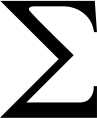
\includegraphics[width=0.225cm]{Bilder/Sigma.png} \nodepart{lower} };
            \pic at ($(#1.lower)-(0,\siz/8)$) {ident=5};
        }
        
        

        % Draw the left input layer nodes
            \foreach \name / \xn in {1,...,\ni}{
            % This is the same as writing \foreach \name / \y in {1/1,2/2,3/3,4/4}
                \node[neuron] (Il-\name) at (\xn*\neuronsep-\neuronsep,\y) [fontscale=15] {$X_{\xn}$};
                \node[above of=Il-\name, node distance=\inout cm] (Inl-\name) {};
                \draw [->,arrows={-Stealth[length=7pt]},densely dotted] (Inl-\name) edge (Il-\name);
            }
            
            \node[fontscale=15] (Il-dot) at ({(\ni+1)*\neuronsep-\neuronsep},\y) {$\dots$};
            
            \node[neuron,fontscale=15] (Il-i) at ({(\ni+2)*\neuronsep-\neuronsep},\y) {$X_{i}$};
            \node[above of=Il-i, node distance=\inout cm] (Inl-i) {};
            \draw [->,arrows={-Stealth[length=7pt]},densely dotted] (Inl-i) edge (Il-i);
            
            

        % Draw the output layer node
            \foreach \name / \xn in {1,...,\no}{
                \node[neuron] (Ol-\xn) at ({(\ni-1)*\neuronsep/2-\neuronsep/2*(\no-1)+(\xn-1)*\neuronsep},\y-\layersep) [fontscale=15] {$Y_{\xn}$};
                
                \node[node distance=\inout cm, below of=Ol-\xn] (Onl) {};
                
                \draw [->,arrows={-Stealth[length=7pt]},densely dotted] (Ol-\xn) edge (Onl);
            }
            
            \node[fontscale=15] (Ol-dot) at ({(\ni-1)*\neuronsep/2-\neuronsep/2*(\no+1)+(\no+1)*\neuronsep},\y-1*\layersep)  {$\dots$};
                
                \node[neuron,fontscale=15] (Ol-o) at ({(\ni-1)*\neuronsep/2-\neuronsep/2*(\no+2)+(\no+2.5)*\neuronsep},\y-1*\layersep)  {$Y_o$};
                \node[node distance=\inout cm, below of=Ol-o] (Onl) {};
                \draw [->,arrows={-Stealth[length=7pt]},densely dotted] (Ol-o) edge (Onl);  
                
              
        % Connect every node in the input layer with the output layer
            \foreach \name / \xn in {1,...,\no,o}{
            \foreach \source in {1,...,\ni,i}
                \draw [->,arrows={-Stealth[length=7pt]}] (Il-\source) edge (Ol-\xn);
            }
                
                
        % Annotate the layers
                \node[annot,right of=Il-i, node distance=\dlsize cm] (il) {\textbf{Eingabe- schicht}};
                \node[annot,below of=il] {\textbf{Ausgabe- schicht}};
        %-----------------------------------------
        %% rechtes Bild

        % Draw the right input layer nodes
                \node[xshift=\dlsize cm] (Ir) at (il) {};
            \foreach \name / \xn in {1,...,\ni}{
        % This is the same as writing \foreach \name / \y in {1/1,2/2,3/3,4/4}
                \node[neuron] (Ir-\name) at ($(Ir)+(\xn*\neuronsep-\neuronsep,0)$) {};
                \node[above of=Ir-\name, node distance=\inout cm] (Inr-\name) {};
                \pic at (Ir-\name) {ident=4};
                \draw [->,arrows={-Stealth[length=7pt]},densely dotted] (Inr-\name) edge (Ir-\name);
            }
            
            \node[fontscale=15] (Ir-dot) at ($(Ir)+({(\ni+1)*\neuronsep-\neuronsep},0)$) {$\dots$};
            
            \node[neuron,fontscale=15] (Ir-i) at ($(Ir)+({(\ni+2)*\neuronsep-\neuronsep},0)$) {};
            \pic at (Ir-i) {ident=4};
            \node[above of=Ir-i, node distance=\inout cm] (Inr-i) {};
            \draw [->,arrows={-Stealth[length=7pt]},densely dotted] (Inr-i) edge (Ir-i);
            
        % Draw the output layer node
            \foreach \name / \xn in {1,...,\no}{
                \neurono[Or-\xn]{$(Ir)+({(\ni-1)*\neuronsep/2-\neuronsep/2*(\no-1)+(\xn-1)*\neuronsep},-\layersep)$}

                \node[node distance=\inout cm, below of=Or-\xn] (Onr) {};
                
                \draw [->,arrows={-Stealth[length=7pt]},densely dotted] (Or-\xn) edge (Onr);
            }
            
             \node[fontscale=15] (Or-dot) at ($(Ir)+({(\ni-1)*\neuronsep/2-\neuronsep/2*(\no+1)+(\no+1)*\neuronsep},-\layersep)$)  {$\dots$};
                
                \neurono[Or-o]{$(Ir)+({(\ni-1)*\neuronsep/2-\neuronsep/2*(\no+2)+(\no+2.5)*\neuronsep},-\layersep)$}
                \node[node distance=\inout cm, below of=Or-o] (Onr) {};
                \draw [->,arrows={-Stealth[length=7pt]},densely dotted] (Or-o) edge (Onr);    
                
        % Connect every node in the input layer with the output layer
            \foreach \name / \xn in {1,...,\no,o}{
            \foreach \source in {1,...,\ni,i}
                \draw [->,arrows={-Stealth[length=7pt]},every node/.style={fill=white,inner sep=1pt,fontscale=7}] 
                (Ir-\source) edge  (Or-\xn);
            }
        
            \draw [fill=white,draw=black, dotted] ($(Ir-1)+(\neuronsep/4-.45,-\layersep*.6)$) rectangle ($(Ir-i)+(\neuronsep/100,-\layersep*.375)$);
                
            \node[fill=white,inner sep=1pt,fontscale=10] at ($(Ir-1)+({(\ni+1)*\neuronsep/2},-\layersep*.5)$) {$\dots\,w_{o,i}\,\dots$};
        
        \end{tikzpicture}
    \caption{SLP das bei der Herleitung der Deltaregel betrachtet wird.}
    \label{fig:SLP_a}
\end{figure}

Zunächst wird die Verarbeitung von Informationen in dem in \autoref{fig:SLP_a} dargestellten Netzwerk betrachtet. Die Information jedes Eingabeneurons $x_i$ wird mit einem Gewicht $w_{oi}$ versehen und an das Ausgabeneuron weitergeleitet. Die Propagierungsfunktion (die in diesem Fall die Summe darstellt) verarbeitet die Eingabe zu Netzeingabe $net_o$
\begin{equation}
net_o= \sum^{i=1}_n w_{oi} \cdot x_i
\end{equation}
und reicht diese an die Aktivierungsfunktion $f_{akt}$ weiter. Das Ergebniss der Aktivierungsfunktion ist dann die Ausgabe $y_o$ des Ausgabeneurons $o$
\begin{equation}
\gls{yo}= f_{akt}(net_o).
\end{equation}
Eine lineare Aktivierungsfunktion ergibt als Ausgabe eine Identität und somit ist
\begin{equation}
y_o= net_o= \sum_{i=1}^n w_{oi} \cdot x_i.
\label{gl:ausgang}
\end{equation}

Nun Soll das Netzwerk mit einer Menge an Lernbeispielen $P$ trainiert werden. Wobei die Menge $\gls{P}$ sich aus der Trainingseingabe $\gls{p}$ und der zugehörigen Lösung $\gls{t}$ also $(p,t)$ zusammensetzt.
Das Ziel des Trainings ist nun, dass die Ausgabe $y$ bei allen Trainingsbeispielen sich der zugehörigen Lösung $t$ möglichst angleicht bzw. die Differenz $\delta$ (auch als Fehler bezeichnet) 
\begin{equation}
\gls{delta}=t-y
\label{gl:delta}
\end{equation}
%
aus Lösung und Ausgabe möglichst klein  wird, also soll formal gelten
\begin{equation*}
\forall p:y \approx t \quad \text{bzw.} \quad \forall p:\delta \approx 0.
\end{equation*}

Bei einem Netzwerk mit zwei Eingabeneuronen und einem Ausgabeneuron (ergo zwei Gewichten) für ein Lernbeispiel eine Fehlerfläche $Err_p(W)$ (dargestellt in \autoref{fig:Fehlerlandschaft}), wobei $W$ die Menge aller Gewichte darstellt.

%\todo{Grafik: Fehlerfläche \citet[80]{dkriesel07}}
\begin{figure}[tb]
    \centering
        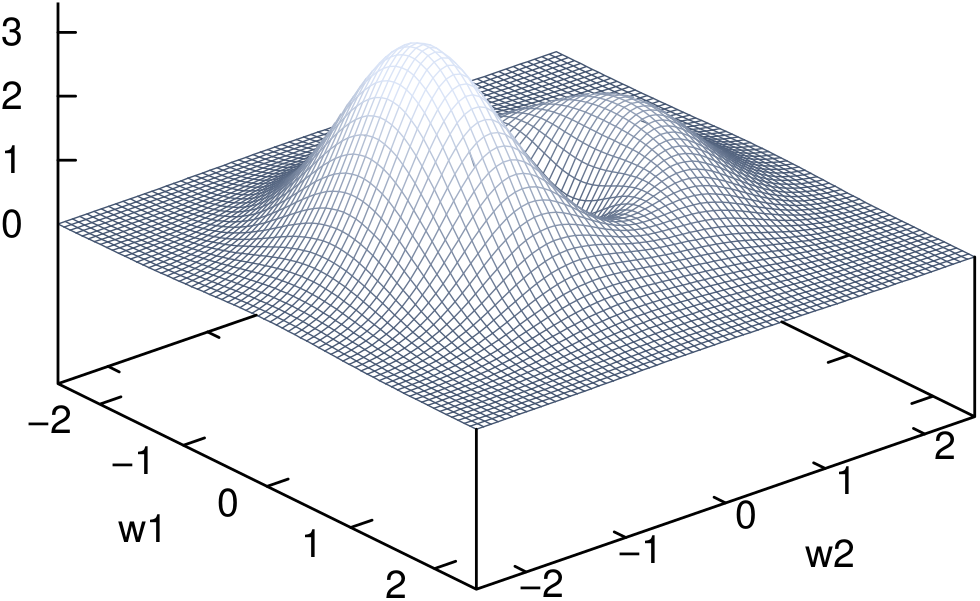
\includegraphics[width=0.5\textwidth]{Bilder/misc/Fehlerlandschaft.png}
    \caption[Beispiel einer Fehlerfläche eines künstlichen neuronalen Netzes]{Beispiel einer Fehlerfläche eines neuronalen Netzes mit zwei trainierbaren Gewichten. Bei weiteren Gewichten entsteht pro Gewicht eine zusätzliche Dimension in der Fehlerlandschaft. Was zu höherer Komplexität und zerklüfteter \glqq Oberfläche\grqq~führt.\protect\footnotemark{}}
    \label{fig:Fehlerlandschaft}
\end{figure}
\addtocounter{footnote}{-1}     %  -1 mal die Gesamtanzahl an Fußnoten in der wrapfigure
\addtocounter{Hfootnote}{-1}    % -1 times total number of footnote(mark)s in the wrapfigure
\wrapfigfoot\footnotetext{\autoref{fig:Fehlerlandschaft} wurde aus \citet[80]{dkriesel07} übernommen.}

Durch Anwendung des Gradientenabstigverfahrens\,\citef[63 f]{dkriesel07} kann nun vom Ausgangspunkt gesehen das nächste Minimum gefunden werden. Mit
\begin{equation}
\Delta w = - \alpha \nabla Err(W)
\end{equation}
erhält man nun die Information wie die Gewichte verändert werden können, um das Fehlerminimum zu finden.
Wobei $\gls{alpha}$ eine Proportionalitätskonstante darstellt, welche für die Schrittweite beim Gradientenabstieg verantwortlich ist.
Um zu erfahren wie jedes Gewicht verändert werden soll muss die Fehlerfunktion $Err(W)$ nach dem entsprechenden Gewicht $w_{oi}$ abgeleitet werden
\begin{equation}
\Delta w_{oi} = - \alpha \frac{\partial Err(W)}{\partial w_{oi}} .
\label{gl:gewaend}
\end{equation}

Die Fehlerfunktion $Err_p(W)$ für ein Trainingsbeispiel $p$ lässt sich auf unterschiedliche Weise bestimmen\,\footnote{\citet[60 f]{dkriesel07} gibt hierfür einige Beispiele an.}, an dieser Stelle wird der quadratische Abstand genutzt. Damit kann die Fehlerfunktion über alle Ausgabeneuronen berechnet werden mit:
\begin{equation}
Err_p(W)= \frac{1}{2} \sum^k_{o=1} (t_{po}-y_{po})^2 .
\end{equation}
Somit reduziert sich die Fehlerfunktion bei der Betrachtung eines Ausgabeneurons $o$ für ein Trainingsbeispiel $p$ zu
\begin{equation}
Err_p(W)= \frac{1}{2} (t_{po}-y_{po})^2 .
\label{gl:errp}
\end{equation}


Dabei entspricht bei dem Onlinelernen der Gesamtfehler $Err(W)$ dem Einzelfehler $Err_p(W)$
\begin{equation}
Err(W)=Err_p(W) 
\end{equation}
und bei dem Offlinelernen müssen die Einzelfehler aufsummiert werden
\begin{equation}
Err(W)= \sum^P_{p=1} Err_p(W). 
\end{equation}

Da in der \autoref{gl:errp} $t_{po}$ konstant ist hängt $Err_p(W)$ nur von $y_{po}$ ab. So kann die Ableitung $\frac{\partial Err_p(W)}{\partial w_{oi}}$ mit der Kettenregel zerlegt werden in
\begin{equation}
\frac{\partial Err_p(W)}{\partial w_{oi}}= \frac{\partial Err_p(W)}{\partial y_{po}} \cdot \frac{\partial y_{po}}{\partial w_{oi}}.
\label{gl:zerlket}
\end{equation}

Durch das Ableiten der \autoref{gl:errp} nach $y_{po}$ und einsetzen von \autoref{gl:delta} erhält man
\begin{equation}
\frac{\partial Err_p(W)}{\partial y_{po}} = -(t_{po}-y_{po}) = - \delta_{po} .
\label{gl:minusdelta}
\end{equation}

Unter Betrachtung der \autoref{gl:ausgang} kann der Ausdruck $ \frac{\partial y_{po}}{\partial w_{oi}}$ nun auch geschrieben werden als 
\begin{equation}
\frac{\partial y_{po}}{\partial w_{oi}} = \frac{\partial \sum\limits_{i=1}^n w_{oi} \cdot x_{pi}}{\partial w_{oi}} .
\label{gl:vor_xi}
\end{equation}
Wobei die abzuleitende Funktion zwar aus vielen Summanden zusammengesetzt ist aber nur der Summand $w_{oi} x_{pi}$ enthält die Variable $w_{oi}$ nach der abgeleitet wird. Es gilt also
\begin{equation}
\frac{\partial y_{po}}{\partial w_{oi}} = x_{pi}.
\label{gl:xi}
\end{equation}
Durch das Einsetzen der \autoref{gl:xi} und \autoref{gl:minusdelta} in \autoref{gl:zerlket} erhält man:
\begin{equation}
\frac{\partial Err_p(W)}{\partial w_{oi}}= - \delta_{po} \cdot x_{pi}.
\label{gl:ze}
\end{equation}
Somit kann mit der \autoref{gl:gewaend} die Deltaregel für das Onlinelernverfahren bestimmt werden:
\begin{equation}
\Delta w_{oi} = \alpha \cdot \delta_{po} \cdot x_{pi} .
\label{gl:fertig_delta}
\end{equation}
Für das Offlinelernverfahren muss noch die Summe über alle Trainingsbeispiele gebildet werden
\begin{equation}
\Delta w_{oi} = \alpha \cdot \sum^P_{p=1} \delta_{po} \cdot x_{pi} .
\end{equation}



%\subsection{Ergebnisse von \citet{Aggarwal2009} und \citet{Panapakidis2016}}\label{sec:andere_ergebnisse}

%\todo{Liste der Märkte aus \citet{Cerjan2013}}

%\todo{Tabellen einfügen und Hinweiß dass SVM keine ANN sind}
\newpage
\subsection{Performancemaße}\label{sec:perfmas}
In diesem Abschnitt werden die Maße zur Evaluierung der Vorhersagegenauigkeit (weiterhin als Performancemaße bezeichnet) aufgeführt die in der Literaturrecherche zur Strompreismodellierung in \autoref{sec:strompreis} und weiterer Literatur\,\citef[5]{Guertler2017} genannt wurden. Hierbei sind $\gls{yi}$ und $\hat{\gls{yih}}_i$ die tatsächlichen und vorhergesagten Preise zum Zeitpunkt $i$ und $\gls{T}$ stellt die Menge aller, bei der Prognose, betrachteten Zeitpunkte dar. Außerdem gibt $\mean{\gls{ym}}$ den Mittelwert der tatsächlichen Preise und $\mean{\gls{ymt}}_{train}$ den Preismittelwert der Trainingsdaten an.

Der Absolute Percentage Error (\gls{APE}) liefert Informationen über die Fehlerverteilung in der Nähe der Null.\,\citef[14\label{foot:Domanski2017}]{Domanski2017}
%
% APE
\begin{equation}
APE= \sum\limits_{i \in T} \frac{\abs{y_i-\hat{y}_i}}{y_i}.
\label{gl:APE}
\end{equation}
%
%
Der Mean Absolute Percentage Error (\gls{MAPE}) gibt einen prozentualen Mittelwert über den Fehlerbetrag an. Da das Ursprungsmaß (in dieser Arbeit als $MAPE_1$ bezeichnet) bei sehr kleinen Preisen einen hohen Werte liefert und bei einem Preis von Null sogar gegen Unendlich gehen wurden Mehrere Verbesserungen vorgeschlagen. Diese äußern sich durch einen Mittelwert über alle gemessenen Preise bei $MAPE_2$ oder durch einen Mittelwert aus der Betragssumme der des tatsächlichen und vorhergesagten Preises bei $sMAPE$ im Nenner. Hierbei steht ein Wert von 0\,\% für eine exakte und Werte um die 10\,\% für eine akkurate Vorhersage.\,\footnote{Vgl. \citet[17]{Bobinaite2016}, \citet[2105]{Amjady2009} und \citet[894]{Lago2018}.}   
% MAPE
\begin{equation}
MAPE_1= \frac{100}{T} \sum\limits_{i \in T} \frac{\abs{y_i-\hat{y}_i}}{y_i},
\label{gl:MAPE_1}
\end{equation}
%
% MAPE
\begin{equation}
MAPE_2= \frac{100}{T} \sum\limits_{i \in T} \frac{\abs{y_i-\hat{y}_i}}{\mean{y}},
\label{gl:MAPE_2}
\end{equation}
%
% sMAPE
\begin{equation}
sMAPE= \frac{100}{T} \sum\limits_{i \in T} \frac{\abs{y_i-\hat{y}_i}}{(\abs{y_i} + \abs{\hat{y}_i}) / 2}.
\label{gl:sMAPE}
\end{equation}
%
Der Mean Squared Error (\gls{MSE}) gibt den quadratischen Mittelwert der der Fehler an und gibt an wie weit die vorhergesagten Daten von den tatsächlichen Werten liegen. Ein kleine Wert deutet auf eine gute vorhersage hin.\,\footnoteref{foot:Domanski2017}
% MSE
\begin{equation}
MSE= \frac{1}{T} \sum\limits_{i \in T} (y_i-\hat{y}_i)^2.
\label{gl:MSE}
\end{equation}
%
%
Der Root Mean Squared Error (\gls{RMSE}) ist die Quadratwurzel des MSE und ist hierdurch sehr ähnlich. Der RMSE weist kleinere Werte auf, der Aussagegehalt ist aber ähnlich zu MSE.
% RMSE
\begin{equation}
RMSE= \sqrt{ \frac{1}{T} \sum\limits_{i \in T} (y_i-\hat{y}_i)^2}.
\label{gl:RMSE}
\end{equation}
%
Der Mean Absolut Error (\gls{MAE}) ist ebenfalls sehr ähnlich zum MSE und damit auch dem RMSE. Weist aber im Vergleich zum RMSE nochmals kleinere Werte auf.
% MAE
\begin{equation}
MAE= \frac{1}{T} \sum\limits_{i \in T} \abs{y_i-\hat{y}_i}.
\label{gl:MAE}
\end{equation}
%
%
Der Normalized Mean Square Error (\gls{NMSE}) ist ein Schätzwert über alle Abweichungen zwischen vorhergesagten und gemessenen Werten. Zeigt ein Modell einen sehr geringen NMSE so weist es eine gute örtliche und zeitliche Performance auf. Andererseits bedeuten hohe $NMSE$-Werte nicht, dass das betrachtete Modell komplett falsch ist.
% NMSE
\begin{gather}
\begin{aligned}
NMSE &= \frac{1}{\Delta^2 T} \sum\limits_{i \in T} (y_i-\hat{y}_i)^2,\\ 
\Delta^2 &= \frac{1}{T-1} \sum\limits_{i \in T} (y_i-\mean{y})^2.\\
\end{aligned}
\label{gl:NMSE}
\end{gather}
%
%
Die Error Variance (\gls{EV}) gibt einen Wert über die nicht erklärten Informationen nach dem Fitten des Modells. Je kleiner der Wert ist desto präziser ist die Vorhersage.\,\citef{Peter2016}
% EV
\begin{equation}
EV= \sigma^2 = \frac{1}{T} \sum\limits_{i \in T} \left ( \frac{\abs{y_i-\hat{y}_i}}{\mean{y}} - MAPE_2  \right ) ^2.
\label{gl:EV}
\end{equation}
%
Pearson Korrelationskoeffizient bewertet die Linearität zwischen der Kovarianz zweier Variablen und dem Produkt der Standardabweichung dieser Variablen. Der Wertebereich dieses Maßes ist [-1,1] und er gibt Auskunft, wie Ähnlich der zeitliche Verlauf zwischen dem tatsächlichen Preis und der Vorhersage ist. Ein Wert von Eins deutet auf eine perfekte vorhersage hin.\,\citef{Davo2016} 
% cor
\begin{equation}
\gls{COR} = \frac{cov(y_i,\hat{y}_i)}{\sqrt{sd(y_i)sd(\hat{y}_i)}} .
\label{gl:cor}
\end{equation}
%
%
Theils Koeffizienten der Ungleichheit \gls{U}[1] und U2 unterscheiden sich in der Anwesenheit bzw. Abwesenheit eines $\hat{y}_i$ im Nenner. Hierbei steht der Wert von Null in beiden fällen für Gleichheit und somit für eine ideale Vorhersage. Bei einem Wert von Eins spricht man von einer maximalen Ungleichheit. Dies kann bei U1 der Fall sein wenn eine negative Proportionalität besteht oder einer der Terme im Nenner Null ist. Bei dem U2 kann dies der Fall sein, wenn die Vorhersagemethode eine \textit{Na\"{i}ve-No-Change-Extrapolation}\,\citef[6]{Lattyak2011} ist oder wenn U2 zu der gleichen Standardabweichung des Prognosefehlers führt wie die Vorhersagemethode.\,\citef[444 f]{Bliemel1973}
% U1
\begin{equation}
U1 = \frac{\sqrt{\frac{1}{T} \sum_{i \in T} (y_i-\hat{y}_i)^2}}{ \sqrt{\frac{1}{T} \sum_{i \in T} y_i^2} + \sqrt{\frac{1}{T} \sum_{i \in T} \hat{y}_i^2}},
\label{gl:U1}
\end{equation}
%
% U2
\begin{equation}
U2 = \frac{\sqrt{\sum_{i \in T} (y_i-\hat{y}_i)^2}}{ \sqrt{ \sum_{i \in T} y_i^2} }.
\label{gl:U2}
\end{equation}
%
%
Das out-of-sample (\gls{R2}) Bestimmtheitsmaß ist dem Relative Absolute Error (\gls{RAE}) sehr ähnlich. Wenn das RAE kleiner 100 und das R$^2$ größer Null ist, so ist die Vorhersagegenauigkeit höher als der historische Mittelwert der Trainingsdaten.
% R²
\begin{equation}
R^2 = 1 -  \frac{\frac{1}{T} \sum_{i \in T} \abs{y_i-\hat{y}_i}^2}{ \frac{1}{T} \sum_{i \in T} \abs{y_i-\mean{y}_{train}}^2 } ,
\label{gl:R2}
\end{equation}
%
%
% RAE
\begin{equation}
RAE = \frac{\frac{1}{T} \sum_{i \in T} \abs{y_i-\hat{y}_i}}{ \frac{1}{T} \sum_{i \in T} \abs{y_i-\mean{y}_{train}} } \cdot 100 .
\label{gl:RAE}
\end{equation}
%
%
Der Absolute Error (\gls{ABS}) und der Relative Error (\gls{REL}) wertet den systematischen Fehler aus. Der Idealwert ist hierbei Null, wobei dies mit einer exakten Vorhersage gleichzusetzen ist. Positive Werte weisen dabei auf eine Überschätzung und negative auf eine Unterschätzung der Vorhersage hin.\,\citef[5 f]{Guertler2017}
%
% ABS
\begin{equation}
ABS= \frac{1}{T} \sum\limits_{i \in T} (\hat{y}_i-y_i),
\label{gl:ABS}
\end{equation}
%
%
% REL
\begin{equation}
REL= \frac{\sum_{i \in T} (\hat{y}_i-y_i)}{\sum_{i \in T} y_i} .
\label{gl:REL}
\end{equation}



%\begin{figure}[!htb]
%    \centering
%        
\pgfplotsset{every axis/.append style={
                label style={font=\footnotesize},
                tick label style={font=\footnotesize},
                x label style={yshift=.5em},
            }}
%%--------------------MAPE-MAE-RAE-------------------------%%
 \begin{tikzpicture}
 
    \def\datafile{Daten/BP/logist/m/BP_logis_m-epochen.dat}
 
    \pgfplotsset{
        %scale only axis,
        minor x tick num=1,
        xmin=0, xmax=51,
        width=15cm,
        height=8cm,
        ylabel style={rotate=180},
        xticklabel style={
            /pgf/number format/precision=3,
            /pgf/number format/fixed,
            x label style={yshift=.5em},
        },
    }
 
    \begin{axis}[
    axis y line*=left,
    xlabel=Epochen,
    ylabel=MAPE,
    y label style={yshift=.5em},
    %xlabel near ticks,
    minor y tick num=1,
    ]
    \addplot[
    mark=none,
    draw=green,
    ] 
    table[
    /pgf/number format/read comma as period,
    x=epochen, 
    y=MAPE_mean, 
    col sep=tab,
    ] {\datafile};
    \label{MAPE-}


       %\addplot[pattern=crosshatch,pattern color=blue!30!white,draw=blue!30!white]{x^2} \closedcycle;
       %\addplot[red,line legend] coordinates {(0,0) (1,1)};
       %\legend{RMSE,U2}
    \end{axis}

    \begin{axis}[
    axis x line=none,
    axis y line*=left,
    ylabel=MAE,
    y label style={yshift=.5em},
    minor y tick num=1,
    ] 
    %\addlegendimage{/pgfplots/refstyle=MAPE}\addlegendentry{MAPE}
    \pgfplotsset{
        every outer y axis line/.style={xshift=-1.2cm}, 
        every tick/.style={xshift=-1.2cm}, 
        every y tick label/.style={xshift=-1.2cm} 
    }
    
    \addplot[
    mark=none,
    draw=purple,
    ] 
    table[
    /pgf/number format/read comma as period,
    x=epochen, 
    y=MAE_mean,
    col sep=tab,
    ] {\datafile};
    \label{MAE-}
    \end{axis}
    
    \begin{axis}[
    axis x line=none,
    axis y line*=right,
    ylabel=RAE,
    y label style={yshift=-.5em},
    minor y tick num=1,
    ] 
    \addlegendimage{/pgfplots/refstyle=MAPE-}\addlegendentry{MAPE}
    \addlegendimage{/pgfplots/refstyle=MAE-}\addlegendentry{MAE}

    \addplot[
    mark=none,
    draw=cyan,
    ] 
    table[
    /pgf/number format/read comma as period,
    x=epochen, 
    y=RAE_mean, 
    col sep=tab,
    ] {\datafile};
    \addlegendentry{RAE}
    \end{axis}

   \end{tikzpicture}
%    \caption{Gegenüberstellung des $MAPE$, des $MAE$ und des $RAE$ wobei auffällt, dass die Maße sich in einem Faktor unterscheiden.}
%    \label{fig:geg_mape_mae_rae}
%\end{figure}

%\begin{figure}[!htb]
%    \centering
%        \pgfplotsset{every axis/.append style={
                label style={font=\footnotesize},
                tick label style={font=\footnotesize},
                x label style={yshift=.5em},
            }}

%%--------------------RMSE-U2----------------------------%%
 \begin{tikzpicture}
 
    \def\datafile{Daten/BP/logist/m/BP_logis_m-epochen.dat}
 
    \pgfplotsset{
        %scale only axis,
        minor x tick num=1,
        xmin=0, xmax=51,
        width=15cm, %\textwidth,
        height=8cm,
        ylabel style={rotate=180},
        xticklabel style={
            /pgf/number format/precision=3,
            /pgf/number format/fixed,
        },
    }
 
    \begin{axis}[
    axis y line*=left,
    xlabel=Epochen,
    ylabel=RMSE,
    y label style={yshift=.5em},
    %xlabel near ticks,
    minor y tick num=1,
    ]
    \addplot[
    mark=none,
    draw=black,
    ] 
    table[
    /pgf/number format/read comma as period,
    x=epochen, 
    y=RMSE_mean, 
    col sep=tab,
    ] {\datafile};
    \label{RMSE-}

    \end{axis}

    \begin{axis}[
    axis x line=none,
    axis y line*=right,
    ylabel=U2,
    y label style={yshift=-.5em},
    minor y tick num=1,
    ] 
    \addlegendimage{/pgfplots/refstyle=RMSE-}\addlegendentry{RMSE}
    %\pgfplotsset{
    %    every outer y axis line/.style={xshift=-1.2cm}, 
    %    every tick/.style={xshift=-1.2cm}, 
    %    every y tick label/.style={xshift=-1.2cm} 
    %}
    
    \addplot[
    mark=none,
    draw=red,
    ] 
    table[
    /pgf/number format/read comma as period,
    x=epochen, 
    y=U2_mean, 
    col sep=tab,
    ] {\datafile};
    \addlegendentry{U2}
    \end{axis}

   \end{tikzpicture}
%    \caption{Die gleiche Beobachtung wie in \autoref{fig:geg_mape_mae_rae} kann auch bei der Gegenüberstellung des $RMSE$ und des $U2$ gemacht werden.}
%    \label{fig:geg_rmse_u2}
%\end{figure}

%\begin{landscape}
%\begin{figure}[!htb]
%    \centering
%        \pgfplotsset{every axis/.append style={
                label style={font=\footnotesize},
                tick label style={font=\footnotesize},
                x label style={yshift=.5em},
            }}
%%--------------------alle-------------------------%%
 \begin{tikzpicture}
 
    \def\datafile{Daten/BP/logist/m/BP_logis_m-epochen.dat}

    \def\xshiftlab{1.1cm}
 
    \pgfplotsset{}
 
    \pgfplotsset{
        %scale only axis,
        minor x tick num=1,
        xmin=0, xmax=51,
        width=15cm, %\textwidth,
        height=13cm,
        ylabel style={rotate=180},
        xticklabel style={
            /pgf/number format/precision=3,
            /pgf/number format/fixed},
        every axis legend/.append style={
        at={(0.5,1.03)},
        anchor=south},
    }
 %%----------------------RMSE-----------------------------%%
    \begin{axis}[
    axis y line*=left,
    xlabel=Epochen,
    ylabel=RMSE,
    y label style={yshift=.5em},
    xlabel near ticks,
    minor y tick num=1,
    ]
    \addplot[
    mark=none,
    draw=black,
    ] 
    table[
    /pgf/number format/read comma as period,
    x=epochen, 
    y=RMSE_mean, 
    col sep=tab,
    ] {\datafile};
    \label{RMSE}
    \end{axis}

%%------------------------U2------------------------------%%
    \begin{axis}[
    axis x line=none,
    axis y line*=left,
    ylabel=U2,
    y label style={yshift=.75em},
    minor y tick num=1,
    ] 
    \pgfplotsset{
        every outer y axis line/.style={xshift=-\xshiftlab*1.2}, 
        every tick/.style={xshift=-\xshiftlab*1.2}, 
        every y tick label/.style={xshift=-\xshiftlab*1.2} 
    }
    
    \addplot[
    mark=none,
    draw=red,
    ] 
    table[
    /pgf/number format/read comma as period,
    x=epochen, 
    y=U2_mean, 
    col sep=tab,
    ] {\datafile};
    \label{U2}
    \end{axis}

%%------------------------REL------------------------------%%
    \begin{axis}[
    axis x line=none,
    axis y line*=left,
    ylabel=REL,
    y label style={yshift=.6em},
    minor y tick num=1,
    ] 
    \pgfplotsset{
        every outer y axis line/.style={xshift=-\xshiftlab*2.3}, 
        every tick/.style={xshift=-\xshiftlab*2.3}, 
        every y tick label/.style={xshift=-\xshiftlab*2.3} 
    }
    
    \addplot[
    mark=none,
    draw=orange,
    ] 
    table[
    /pgf/number format/read comma as period,
    x=epochen, 
    y=REL_mean, 
    col sep=tab,
    ] {\datafile};
    \label{REL}
    \end{axis}

%%------------------------ABS------------------------------%%
    \begin{axis}[
    axis x line=none,
    axis y line*=left,
    ylabel=ABS,
    y label style={yshift=.6em},
    minor y tick num=1,
    ] 
    \pgfplotsset{
        every outer y axis line/.style={xshift=-\xshiftlab*3.45}, 
        every tick/.style={xshift=-\xshiftlab*3.45}, 
        every y tick label/.style={xshift=-\xshiftlab*3.45} 
    }
    
    \addplot[
    mark=none,
    draw=lime,
    ] 
    table[
    /pgf/number format/read comma as period,
    x=epochen, 
    y=ABS_mean, 
    col sep=tab,
    ] {\datafile};
    \label{ABS}
    \end{axis}

%%------------------------EV------------------------------%%
    \begin{axis}[
    axis x line=none,
    axis y line*=left,
    ylabel=EV,
    y label style={yshift=.5em},
    minor y tick num=1,
    ] 
    \pgfplotsset{
        every outer y axis line/.style={xshift=-\xshiftlab*4.45}, 
        every tick/.style={xshift=-\xshiftlab*4.45}, 
        every y tick label/.style={xshift=-\xshiftlab*4.45} 
    }
    
    \addplot[
    mark=none,
    draw=brown,
    ] 
    table[
    /pgf/number format/read comma as period,
    x=epochen, 
    y=EV_mean, 
    col sep=tab,
    ] {\datafile};
    \label{EV}
    \end{axis}





%%----------------------sMAPE-----------------------------%%
    \begin{axis}[
    axis x line=none,
    axis y line*=right,
    %xlabel=Epochen,
    ylabel=sMAPE,
    y label style={yshift=-.5em},
    minor y tick num=1,
    ]
    \addplot[
    mark=none,
    draw=magenta,
    ] 
    table[
    /pgf/number format/read comma as period,
    x=epochen, 
    y=sMAPE_mean, 
    col sep=tab,
    ] {\datafile};
    \label{sMAPE}
    \end{axis}

%%----------------------MAPE-----------------------------%%
    \begin{axis}[
    axis x line=none,
    axis y line*=right,
    %xlabel=Epochen,
    ylabel=MAPE,
    y label style={yshift=-.5em},
    minor y tick num=1,
    ]
    
    \pgfplotsset{
        every outer y axis line/.style={xshift=\xshiftlab}, 
        every tick/.style={xshift=\xshiftlab}, 
        every y tick label/.style={xshift=\xshiftlab} 
    }
    
    \addplot[
    mark=none,
    draw=green,
    ] 
    table[
    /pgf/number format/read comma as period,
    x=epochen, 
    y=MAPE_mean, 
    col sep=tab,
    ] {\datafile};
    \label{MAPE}
    \end{axis}

%%----------------------MAE-----------------------------%%
    \begin{axis}[
    axis x line=none,
    axis y line*=right,
    ylabel=MAE,
    y label style={yshift=-.85em},
    minor y tick num=1,
    ] 
    %\addlegendimage{/pgfplots/refstyle=MAPE}\addlegendentry{MAPE}
    \pgfplotsset{
        every outer y axis line/.style={xshift=\xshiftlab*2}, 
        every tick/.style={xshift=\xshiftlab*2}, 
        every y tick label/.style={xshift=\xshiftlab*2} 
    }
    
    \addplot[
    mark=none,
    draw=purple,
    ] 
    table[
    /pgf/number format/read comma as period,
    x=epochen, 
    y=MAE_mean,
    col sep=tab,
    ] {\datafile};
    \label{MAE}
    \end{axis}

%%----------------------RAE-----------------------------%%
    \begin{axis}[
    axis x line=none,
    axis y line*=right,
    ylabel=RAE,
    y label style={yshift=-.5em},
    minor y tick num=1,
    ]

    \pgfplotsset{
        every outer y axis line/.style={xshift=\xshiftlab*3}, 
        every tick/.style={xshift=\xshiftlab*3}, 
        every y tick label/.style={xshift=\xshiftlab*3} 
    }

    \addplot[
    mark=none,
    draw=cyan,
    ] 
    table[
    /pgf/number format/read comma as period,
    x=epochen, 
    y=RAE_mean, 
    col sep=tab,
    ] {\datafile};
    \label{RAE}
    \end{axis}

%%----------------------R²-----------------------------%%
    \begin{axis}[
    axis x line=none,
    axis y line*=right,
    ylabel=R$^2$,
    y dir=reverse,
    y label style={yshift=-.5em},
    minor y tick num=1,
    legend columns=10,
    ]
    
    \addlegendimage{/pgfplots/refstyle=RMSE}\addlegendentry{RMSE}
    \addlegendimage{/pgfplots/refstyle=U2}\addlegendentry{U2}
    \addlegendimage{/pgfplots/refstyle=REL}\addlegendentry{REL}
    \addlegendimage{/pgfplots/refstyle=ABS}\addlegendentry{ABS}
    \addlegendimage{/pgfplots/refstyle=EV}\addlegendentry{EV}
    \addlegendimage{/pgfplots/refstyle=sMAPE}\addlegendentry{sMAPE}
    \addlegendimage{/pgfplots/refstyle=MAPE}\addlegendentry{MAPE}
    \addlegendimage{/pgfplots/refstyle=MAE}\addlegendentry{MAE}
    \addlegendimage{/pgfplots/refstyle=RAE}\addlegendentry{RAE}

    \pgfplotsset{
        every outer y axis line/.style={xshift=\xshiftlab*4}, 
        every tick/.style={xshift=\xshiftlab*4}, 
        every y tick label/.style={xshift=\xshiftlab*4} 
    }

    \addplot[
    mark=none,
    draw=blue,
    ] 
    table[
    /pgf/number format/read comma as period,
    x=epochen, 
    y=R2_mean, 
    col sep=tab,
    ] {\datafile};
    \addlegendentry{R2}
    \end{axis}

   \end{tikzpicture}
%    \caption{Dargestellt ist die Messung der optimalen Epochenanzahl eines MLPs mit Bias-Neuron welches mit dem BP-Verfahren trainiert wird und eine logistische Aktivierungsfunktion besitzt. Dieser Graph dient der Gegenüberstellung aller in dieser Arbeit betrachteten Performancemaße.}
%    \label{fig:geg_alle}
%\end{figure}
%\end{landscape}

%-----------------------------------------------------------------------------------

\newpage
\subsection{Überblick und Benutzung der Programme}\label{sec:program}

Die programmiertechnischen Umsetzungen der beschriebenen Algorithmen befinden sich im digitalen Anhang auf der CD. In dem Ordner \verb|Programme\Datensatz\| befindet sich der Ordner \verb|raw| und die Datei \verb|Datensatz.dta|. In dem Ordner \verb|raw| befinden sich die Rohdaten in Excel-Format und die Datei \verb|Datensatz.dta| beinhaltet den Datensatz dieser Arbeit und kann direkt in Stata eingebunden werden.

In dem Ordner \verb|Programme\Stata\| befinden sich die Ordner \verb|ann|, \verb|sub| und die Dateien \verb|cr_annlib.do| und \verb|lannlib.mlib|. Die Datei \verb|cr_annlib.do| ist eine Bibliothek, welche die einzelnen Netzwerke enthält. Die einzelnen Netzwerke befinden sich in der entsprechenden \verb|*.mata| Datei in dem Ordner \verb|ann|. Die Datei \verb|lannlib.mlib| wird auf Grundlage von \verb|cr_annlib.do| automatisch erzeugt und dient der schnelleren Kalkulation der Netzwerke.

In dem Ordner \verb|sub| befinden sich die Programme zum herausfinden der optimalen Parameter (\verb|optimize_*.do|) und Evaluation (\verb|evaluate_*.do|) der einzelnen Netzwerke.
Für jeden Lernalgorithmus gibt es eine eigene Datei. Wobei die Dateien \verb|optimize_*.do| und \verb|evaluate_*.do| ähnlich strukturiert sind. 
Es werden nun die Codezeilen angegeben, die angepasst werden müssen damit die Programme gestartet werden können.\\

\begin{Verbatim}[commandchars=\\\{\}]
\textbf{optimize_*.do:}
\end{Verbatim}
Bevor ein Netzwerk die gewünschte Ausgabe liefern kann müssen zunächst die optimalen Werte der Lernalgorithmen bestimmt werden. Die Nachfolgend beschriebenen Programme dienen diesem Zweck. Es werden mehrere Schleifen durchlaufen wobei der zu untersuchende Parameter in einer bestimmten Schrittweite Verändert wird. Die Programme speichern dabei die berechneten Werte, zur nachfolgenden Auswertung, in eine Ausgabedatei im Excel-Format.

Bei beiden Lernalgorithmen muss zunächst der Ordnerpfad angegeben werden in dem sich die \verb|cr_annlib.do| befindet.\footnote{Um mögliche Sprachbarrieren abzubauen sind die Kommentare in den Quelldateien in englischer Sprache verfasst.}

{
\setstretch{1} 
\begin{lstlisting}[firstnumber=4]
//-----------------------------
// Ordner in dem sich cr_annlib.do befindet
cd "E:\Programme\Stata"
//-----------------------------
\end{lstlisting}
}

\newpage
Als nächstes muss der Ordnerpfad angegeben werden, in dem die Ausgabedatei abgespeichert wird. \farbig{Dieser Ordner muss vor dem Start der do-File existieren!}


{
\setstretch{1} 
\begin{lstlisting}[firstnumber=225]
//-----------------------------
// Speicherort der Ausgabedatei
path = "E:\Programme\Results"
//-----------------------------
\end{lstlisting}
}

Anschließend wird der Speicherort des Datensatzes angegeben.

{
\setstretch{1} 
\begin{lstlisting}[firstnumber=257]
//-----------------------------
// Speicherort des Datensatzes
data = sample_conv(`"use "E:\Programme\Datensatz\Datensatz.dta""',variable,datarange)
//-----------------------------
\end{lstlisting}
}

Dann wird die gewünschte Netzwerkkonstellation gewählt.
\begin{Verbatim}
optimize_mlp_BP.do:
\end{Verbatim}
{
\setstretch{1} 
\begin{lstlisting}[firstnumber=214]
//-----------------------------
// Konstellation wählen
ANN = 1 //"mlp_BP_sig"
//ANN = 2 //"mlp_BP_sig_bias"
//ANN = 3 //"mlp_BP_tanh"
//ANN = 4 //"mlp_BP_tanh_bias"
//-----------------------------
\end{lstlisting}
}

\begin{Verbatim}
optimize_mlp_LM.do:
\end{Verbatim}
{
\setstretch{1} 
\begin{lstlisting}[firstnumber=214]
//-----------------------------
// Konstellation wählen
//ANN = 1 //"mlp_LM_sig"
ANN = 2 //"mlp_LM_sig_bias"
//ANN = 3 //"mlp_LM_tanh"
//ANN = 4 //"mlp_LM_tanh_bias"
//-----------------------------
\end{lstlisting}
}

Dies geschieht indem die Netzwerkkonstellation die nicht gewünscht sind mit \verb|//| auskommentiert werden. Es kann nur eine Konstellation gewählt sein. In dem dargestellten Ausschnitt der \verb|optimize_mlp_BP.do| Datei ist das Netzwerk in Zeile \verb|215| ausgewählt und im Ausschnitt der \verb|optimize_mlp_LM.do| Datei ist das Netzwerk in Zeile \verb|216| ausgewählt.

Nachfolgend werden, abhängig vom Lernalgorithmus die Netzwerkparameter eingestellt.

\begin{Verbatim}
optimize_mlp_BP.do:
\end{Verbatim}
{
\setstretch{1} 
\begin{lstlisting}[firstnumber=278]
//-----------------------------
// Anfangswerte
n.ineuron	= length(variable) // Anzahl der Eingabeneuronen
n.hneuron	= 5                // Anzahl verdeckter Neuronen
n.oneuron	= 1                // Anzahl der Ausgabeneuronen
n.lrate   = 0.83             // Lernrate
//epochen		= 1           // Anzahl der Epochen
//-----------------------------
\end{lstlisting}
}

\begin{Verbatim}
optimize_mlp_LM.do:
\end{Verbatim}
{
\setstretch{1} 
\begin{lstlisting}[firstnumber=278]
//-----------------------------
// Anfangswerte
n.ineuron	= length(variable) // Anzahl der Eingabeneuronen
//n.hneuron	= 13          // Anzahl verdeckter Neuronen
n.oneuron	= 1                // Anzahl der Ausgabeneuronen
n.epochen	= 1                // Maximale Anzahl Iterationen
n.lm		= 0.1              // Abklingfaktor
n.mo = n.mh = 0.01           // Kombinationskoeffizienten
n.Es_max	= 0.0001           // Maximaler Fehler
n.train   = train            // Trainingsbeispiele
n.result_tr = train_raw[1+24::rows(train_raw),1] // Lösungen für Trainingsbeispiele
//-----------------------------
\end{lstlisting}
}

Wobei Parameter deren optimale Werte zu untersuchen sind, an dieser Stelle auskommentiert werden (in \verb|optimize_mlp_BP.do| Zeile \verb|283| und in \verb|optimize_mlp_LM.do| Zeile \verb|280|).
Diese Parameter werden schließlich innerhalb der Berechnungsschleife eingefügt.

\begin{Verbatim}
optimize_mlp_BP.do:
\end{Verbatim}
{
\setstretch{1} 
\begin{lstlisting}[firstnumber=300]
//-----------------------------
// Beispiel: "Parameter" = rate
epochen	= rate
//-----------------------------
\end{lstlisting}
}

\begin{Verbatim}
optimize_mlp_LM.do:
\end{Verbatim}
{
\setstretch{1} 
\begin{lstlisting}[firstnumber=300]
//-----------------------------
// Beispiel: "Parameter" = rate
n.hneuron	= rate
//-----------------------------
\end{lstlisting}
}

Abschließend werden der Anfangs-, Endwert und Schrittweite der zu untersuchenden Parameter eingestellt und die Anzahl an Durchgängen über die das Ergebnis gemittelt wird festgelegt.

{
\setstretch{1} 
\begin{lstlisting}[firstnumber=270]
//-----------------------------
// Untersuchungseinstellungen
start  = 1  // Anfangswert
ende   = 20 // Endwert
step   = 1  // Schrittweite
rounds = 20 // Mittelwert über
//-----------------------------
\end{lstlisting}
}

Nachdem alle Einstellungen durchgeführt wurden kann die do-File im Stata-Editor mit der Tastenkombination \verb|[Strg] + [D]| ausgeführt werden. Wenn der erste Wert berechnet wurde, wird im angegebenen Pfad eine Excel-Datei mit dem aktuellen Datum erstellt und der Wert dort gespeichert. Die Reiter der Excel-Dateien werden nach der Stunde benannt zu der die Messung begonnen hat. Jeder weitere Wert wird in dem gleichen Reiter gespeichert. Nachdem 200 Werte in einer Datei gesichert wurden, wird eine neue Datei erstellt, um die Zugriffszeiten bei der Berechnung zu minimieren.\\

%\newpage

\begin{Verbatim}[commandchars=\\\{\}]
\textbf{evaluate_*.do:}
\end{Verbatim}
Nachdem die optimalen Parameter gefunden sind können die Netzwerke evaluiert werden. Die nachfolgend beschriebenen Dateien bieten die Möglichkeit die vorhergesagten Werte in eine Ausgabedatei im Excel-Format abzuspeichern.
Die Einstellungen der einzelnen Pfade ist analog zu der Beschreibung der \verb|optimize_*.do| Dateien. Um Verwirrungen vorzubeugen werden hier die Einstellungen nochmals vorgestellt, da sich einige Codezeilen unterscheiden.

Bei beiden Lernalgorithmen muss zunächst der Ordnerpfad angegeben werden in dem sich die \verb|cr_annlib.do| befindet.

{
\setstretch{1} 
\begin{lstlisting}[firstnumber=4]
//-----------------------------
// Ordner in dem sich cr_annlib.do befindet
cd "E:\Programme\Stata"
//-----------------------------
\end{lstlisting}
}

%\newpage
Als nächstes muss der Ordnerpfad angegeben werden, in dem die Ausgabedatei abgespeichert wird. \farbig{Dieser Ordner muss vor dem Start der do-File existieren!}

{
\setstretch{1} 
\begin{lstlisting}[firstnumber=273]
//-----------------------------
// Speicherort der Ausgabedatei
path = "E:\Programme\Results"
//-----------------------------
\end{lstlisting}
}

Anschließend wird der Speicherort des Datensatzes angegeben.

{
\setstretch{1} 
\begin{lstlisting}[firstnumber=305]
//-----------------------------
// Speicherort des Datensatzes
data = sample_conv(`"use "E:\Programme\Datensatz\Datensatz.dta""',variable,datarange)
//-----------------------------
\end{lstlisting}
}

Dann wird die gewünschte Netzwerkkonstellation gewählt.
\begin{Verbatim}
evaluate_mlp_BP.do:
\end{Verbatim}
{
\setstretch{1} 
\begin{lstlisting}[firstnumber=262]
//-----------------------------
// Konstellation wählen
ANN = 1 //"mlp_BP_sig"
//ANN = 2 //"mlp_BP_sig_bias"
//ANN = 3 //"mlp_BP_tanh"
//ANN = 4 //"mlp_BP_tanh_bias"
//-----------------------------
\end{lstlisting}
}

\newpage

\begin{Verbatim}
evaluate_mlp_LM.do:
\end{Verbatim}
{
\setstretch{1} 
\begin{lstlisting}[firstnumber=262]
//-----------------------------
// Konstellation wählen
//ANN = 1 //"mlp_LM_sig"
ANN = 2 //"mlp_LM_sig_bias"
//ANN = 3 //"mlp_LM_tanh"
//ANN = 4 //"mlp_LM_tanh_bias"
//-----------------------------
\end{lstlisting}
}

Dies geschieht indem die Netzwerkkonstellation die nicht gewünscht sind mit \verb|//| auskommentiert werden. Es kann nur eine Konstellation gewählt sein. In dem dargestellten Ausschnitt der \verb|optimize_mlp_BP.do| Datei ist das Netzwerk in Zeile \verb|263| ausgewählt und im Ausschnitt der \verb|optimize_mlp_LM.do| Datei ist das Netzwerk in Zeile \verb|264| ausgewählt.

Nachfolgend werden, abhängig vom Lernalgorithmus die Netzwerkparameter eingestellt. Wobei hier die ermittelten optimalen Parameter eingetragen werden. Durch die Anzahl der Neuinitialisierungen kann festgelegt werden wie oft ein Netzwerk mit den gleichen Parametern initialisiert wird. Dabei wird bei jeder Neuinitialisierung die berechnete Prognose gespeichert.

\begin{Verbatim}
evaluate_mlp_BP.do:
\end{Verbatim}
{
\setstretch{1} 
\begin{lstlisting}[firstnumber=318]
//-----------------------------
// Anfangswerte
n.ineuron	= length(variable) // Anzahl der Eingabeneuronen
n.hneuron	= 5                // Anzahl verdeckter Neuronen
n.oneuron	= 1                // Anzahl der Ausgabeneuronen
n.lrate   = 0.83             // Lernrate
epochen   = 27               // Anzahl der Epochen
rounds    = 20			    // Anzahl der Neuinitialisierungen
//-----------------------------
\end{lstlisting}
}

\begin{Verbatim}
evaluate_mlp_LM.do:
\end{Verbatim}
{
\setstretch{1} 
\begin{lstlisting}[firstnumber=318]
//-----------------------------
// Anfangswerte
n.ineuron	= length(variable) // Anzahl der Eingabeneuronen
n.hneuron	= 13               // Anzahl verdeckter Neuronen
n.oneuron	= 1                // Anzahl der Ausgabeneuronen
n.epochen	= 10               // Maximale Anzahl Iterationen
n.lm		= 0.1              // Abklingfaktor
n.mo = n.mh = 0.01           // Kombinationskoeffizienten
n.Es_max	= 0.0001           // Maximaler Fehler
n.train   = train            // Trainingsbeispiele
n.result_tr = train_raw[1+24::rows(train_raw),1] // Lösungen für Trainingsbeispiele
rounds    = 20			    // Anzahl der Neuinitialisierungen
//-----------------------------
\end{lstlisting}
}

Nachdem alle Einstellungen durchgeführt wurden kann die do-File im Stata-Editor mit der Tastenkombination \verb|[Strg] + [D]| ausgeführt werden. Wenn der erste Wert berechnet wurde, wird im angegebenen Pfad eine Excel-Datei mit dem aktuellen Datum erstellt und der Wert dort gespeichert. Die Reiter der Excel-Dateien werden nach der Stunde benannt zu der die Messung begonnen hat. Jeder weitere Wert wird in dem gleichen Reiter gespeichert. Wobei alle Prognosen in einem separaten Reiter gesichert werden. Die Benennung der Prognosen erfolgt durch aufsteigende Ziffern, die der Neuinitialisierung entsprechen in der die Prognose erstellt wurde.